% Options for packages loaded elsewhere
\PassOptionsToPackage{unicode}{hyperref}
\PassOptionsToPackage{hyphens}{url}
%
\documentclass[
]{book}
\usepackage{amsmath,amssymb}
\usepackage{iftex}
\ifPDFTeX
  \usepackage[T1]{fontenc}
  \usepackage[utf8]{inputenc}
  \usepackage{textcomp} % provide euro and other symbols
\else % if luatex or xetex
  \usepackage{unicode-math} % this also loads fontspec
  \defaultfontfeatures{Scale=MatchLowercase}
  \defaultfontfeatures[\rmfamily]{Ligatures=TeX,Scale=1}
\fi
\usepackage{lmodern}
\ifPDFTeX\else
  % xetex/luatex font selection
\fi
% Use upquote if available, for straight quotes in verbatim environments
\IfFileExists{upquote.sty}{\usepackage{upquote}}{}
\IfFileExists{microtype.sty}{% use microtype if available
  \usepackage[]{microtype}
  \UseMicrotypeSet[protrusion]{basicmath} % disable protrusion for tt fonts
}{}
\makeatletter
\@ifundefined{KOMAClassName}{% if non-KOMA class
  \IfFileExists{parskip.sty}{%
    \usepackage{parskip}
  }{% else
    \setlength{\parindent}{0pt}
    \setlength{\parskip}{6pt plus 2pt minus 1pt}}
}{% if KOMA class
  \KOMAoptions{parskip=half}}
\makeatother
\usepackage{xcolor}
\usepackage{color}
\usepackage{fancyvrb}
\newcommand{\VerbBar}{|}
\newcommand{\VERB}{\Verb[commandchars=\\\{\}]}
\DefineVerbatimEnvironment{Highlighting}{Verbatim}{commandchars=\\\{\}}
% Add ',fontsize=\small' for more characters per line
\usepackage{framed}
\definecolor{shadecolor}{RGB}{248,248,248}
\newenvironment{Shaded}{\begin{snugshade}}{\end{snugshade}}
\newcommand{\AlertTok}[1]{\textcolor[rgb]{0.94,0.16,0.16}{#1}}
\newcommand{\AnnotationTok}[1]{\textcolor[rgb]{0.56,0.35,0.01}{\textbf{\textit{#1}}}}
\newcommand{\AttributeTok}[1]{\textcolor[rgb]{0.13,0.29,0.53}{#1}}
\newcommand{\BaseNTok}[1]{\textcolor[rgb]{0.00,0.00,0.81}{#1}}
\newcommand{\BuiltInTok}[1]{#1}
\newcommand{\CharTok}[1]{\textcolor[rgb]{0.31,0.60,0.02}{#1}}
\newcommand{\CommentTok}[1]{\textcolor[rgb]{0.56,0.35,0.01}{\textit{#1}}}
\newcommand{\CommentVarTok}[1]{\textcolor[rgb]{0.56,0.35,0.01}{\textbf{\textit{#1}}}}
\newcommand{\ConstantTok}[1]{\textcolor[rgb]{0.56,0.35,0.01}{#1}}
\newcommand{\ControlFlowTok}[1]{\textcolor[rgb]{0.13,0.29,0.53}{\textbf{#1}}}
\newcommand{\DataTypeTok}[1]{\textcolor[rgb]{0.13,0.29,0.53}{#1}}
\newcommand{\DecValTok}[1]{\textcolor[rgb]{0.00,0.00,0.81}{#1}}
\newcommand{\DocumentationTok}[1]{\textcolor[rgb]{0.56,0.35,0.01}{\textbf{\textit{#1}}}}
\newcommand{\ErrorTok}[1]{\textcolor[rgb]{0.64,0.00,0.00}{\textbf{#1}}}
\newcommand{\ExtensionTok}[1]{#1}
\newcommand{\FloatTok}[1]{\textcolor[rgb]{0.00,0.00,0.81}{#1}}
\newcommand{\FunctionTok}[1]{\textcolor[rgb]{0.13,0.29,0.53}{\textbf{#1}}}
\newcommand{\ImportTok}[1]{#1}
\newcommand{\InformationTok}[1]{\textcolor[rgb]{0.56,0.35,0.01}{\textbf{\textit{#1}}}}
\newcommand{\KeywordTok}[1]{\textcolor[rgb]{0.13,0.29,0.53}{\textbf{#1}}}
\newcommand{\NormalTok}[1]{#1}
\newcommand{\OperatorTok}[1]{\textcolor[rgb]{0.81,0.36,0.00}{\textbf{#1}}}
\newcommand{\OtherTok}[1]{\textcolor[rgb]{0.56,0.35,0.01}{#1}}
\newcommand{\PreprocessorTok}[1]{\textcolor[rgb]{0.56,0.35,0.01}{\textit{#1}}}
\newcommand{\RegionMarkerTok}[1]{#1}
\newcommand{\SpecialCharTok}[1]{\textcolor[rgb]{0.81,0.36,0.00}{\textbf{#1}}}
\newcommand{\SpecialStringTok}[1]{\textcolor[rgb]{0.31,0.60,0.02}{#1}}
\newcommand{\StringTok}[1]{\textcolor[rgb]{0.31,0.60,0.02}{#1}}
\newcommand{\VariableTok}[1]{\textcolor[rgb]{0.00,0.00,0.00}{#1}}
\newcommand{\VerbatimStringTok}[1]{\textcolor[rgb]{0.31,0.60,0.02}{#1}}
\newcommand{\WarningTok}[1]{\textcolor[rgb]{0.56,0.35,0.01}{\textbf{\textit{#1}}}}
\usepackage{longtable,booktabs,array}
\usepackage{calc} % for calculating minipage widths
% Correct order of tables after \paragraph or \subparagraph
\usepackage{etoolbox}
\makeatletter
\patchcmd\longtable{\par}{\if@noskipsec\mbox{}\fi\par}{}{}
\makeatother
% Allow footnotes in longtable head/foot
\IfFileExists{footnotehyper.sty}{\usepackage{footnotehyper}}{\usepackage{footnote}}
\makesavenoteenv{longtable}
\usepackage{graphicx}
\makeatletter
\def\maxwidth{\ifdim\Gin@nat@width>\linewidth\linewidth\else\Gin@nat@width\fi}
\def\maxheight{\ifdim\Gin@nat@height>\textheight\textheight\else\Gin@nat@height\fi}
\makeatother
% Scale images if necessary, so that they will not overflow the page
% margins by default, and it is still possible to overwrite the defaults
% using explicit options in \includegraphics[width, height, ...]{}
\setkeys{Gin}{width=\maxwidth,height=\maxheight,keepaspectratio}
% Set default figure placement to htbp
\makeatletter
\def\fps@figure{htbp}
\makeatother
\setlength{\emergencystretch}{3em} % prevent overfull lines
\providecommand{\tightlist}{%
  \setlength{\itemsep}{0pt}\setlength{\parskip}{0pt}}
\setcounter{secnumdepth}{5}
\usepackage{booktabs}
\ifLuaTeX
  \usepackage{selnolig}  % disable illegal ligatures
\fi
\usepackage[]{natbib}
\bibliographystyle{plainnat}
\usepackage{bookmark}
\IfFileExists{xurl.sty}{\usepackage{xurl}}{} % add URL line breaks if available
\urlstyle{same}
\hypersetup{
  pdftitle={Asignatura Series de Tiempo},
  pdfauthor={Brayan Hernandez Cardona - Adriana Avila - WILLIAM ROJAS CARABALI},
  hidelinks,
  pdfcreator={LaTeX via pandoc}}

\title{Asignatura Series de Tiempo}
\author{Brayan Hernandez Cardona - Adriana Avila - WILLIAM ROJAS CARABALI}
\date{2024-11-04}

\begin{document}
\maketitle

{
\setcounter{tocdepth}{1}
\tableofcontents
}
\chapter{Acerca de este libro}\label{acerca-de-este-libro}

Este libro recopila los resultados más relevantes obtenidos durante el curso de series de tiempo de la Maestría en Ciencia de Datos, incluyendo análisis, modelos y predicciones.

Los datos para la realización de este book son suministrados por una empresa del sector retail en el ambito de electrónica de la cual se tiene el permiso para su uso durante esta asignatura.

\section{Introducción}\label{introducciuxf3n}

En el actual panorama empresarial, caracterizado por una dinámica competitiva intensa y fluctuaciones del mercado, la capacidad de previsión se erige como un factor determinante para la sostenibilidad y el crecimiento de las organizaciones. La predicción precisa de las ventas reviste una importancia capital para la optimización de recursos, la planificación estratégica y la toma de decisiones en áreas clave como la gestión de inventarios, la producción y el marketing. En este contexto, el análisis de series temporales se posiciona como una metodología cuantitativa robusta con un amplio potencial para identificar patrones, tendencias y comportamientos recurrentes en los datos de ventas, permitiendo la generación de pronósticos confiables y la anticipación a las fluctuaciones de la demanda.

Esta obra se propone profundizar en el marco teórico-práctico del análisis de series temporales aplicado a la predicción de ventas. A lo largo de sus capítulos, se abordarán con rigor los fundamentos matemáticos y estadísticos de esta disciplina, se examinarán las principales técnicas de modelado y se presentarán casos de estudio.

\begin{Shaded}
\begin{Highlighting}[]
\CommentTok{\#install.packages("bookdown")}
\NormalTok{bookdown}\SpecialCharTok{::}\FunctionTok{render\_book}\NormalTok{()}
\end{Highlighting}
\end{Shaded}

\begin{Shaded}
\begin{Highlighting}[]
\NormalTok{bookdown}\SpecialCharTok{::}\FunctionTok{serve\_book}\NormalTok{()}
\end{Highlighting}
\end{Shaded}

\chapter{Pronóstico de Ventas en empresa Retail}\label{pronuxf3stico-de-ventas-en-empresa-retail}

\section{Optimizando el Futuro del Retail}\label{optimizando-el-futuro-del-retail}

Este proyecto se centra en el análisis y pronóstico de ventas de una empresa en el sector retail, una pequeña cadena de tiendas de electrónica con 3 sucursales ubicadas en diferentes ciudades de Colombia. El conjunto de datos utilizado contiene información detallada de las transacciones realizadas en cada tienda durante los años 2017 y 2020.

\section{Estructura del dataset}\label{estructura-del-dataset}

En nuestro dataset se encuentra información de las transacciones de ventas de 4 años comprendidos entre el inicio de 2017 y finales de 2020. En el cual disponemos de la siguiente información:

\begin{itemize}
\tightlist
\item
  \textbf{Fecha y hora de la transacción:} Permite analizar patrones de compra a lo largo del tiempo.
\item
  \textbf{Nombre de la sucursal:} Permite comparar el rendimiento de las diferentes sucursales.
\item
  \textbf{Categoría del producto:} (repuestos, accesorios, electrodomesticos, servicios) Facilita el análisis de la demanda por categorías.
\item
  \textbf{ID del producto:} Permite comparar el rendimiento de los diferentes productos.
\item
  \textbf{Precio del producto:} Útil para analizar la relación entre precio y volumen de ventas.
\item
  \textbf{Cantidad vendida:} Permite calcular las ventas totales y el rendimiento de cada producto.
\item
  \textbf{Método de pago:} (e.g., efectivo, tarjeta de crédito, tarjeta débito) Permite identificar tendencias en los métodos de pago.
\item
  \textbf{Descuentos y promociones aplicadas:} Permite evaluar la efectividad de las estrategias promocionales.
\end{itemize}

\subsection{¿Por qué es crucial pronosticar las ventas?}\label{por-quuxe9-es-crucial-pronosticar-las-ventas}

En un entorno minorista altamente competitivo, la capacidad de anticipar la demanda futura es fundamental para el éxito de las pequeñas empresas. Un pronóstico con buena asertividad permite:

\begin{itemize}
\tightlist
\item
  \textbf{Optimizar la gestión de inventario:} Evitar el exceso de stock y las roturas de stock, minimizando costos de almacenamiento y maximizando la disponibilidad de productos.
\item
  \textbf{Planificar las necesidades de personal:} Asignar el número adecuado de empleados en cada tienda y en cada turno, optimizando la atención al cliente y la eficiencia operativa.
\item
  \textbf{Maximizar la rentabilidad:} Ajustar las estrategias de precios y promociones en función de la demanda prevista, aumentando las ventas y la rentabilidad.
\item
  \textbf{Tomar decisiones estratégicas:} Identificar tendencias de consumo, evaluar la efectividad de las estrategias de marketing, y planificar la expansión a nuevas ubicaciones.
\end{itemize}

\subsection{¿Qué podemos aportar desde la ciencia de datos?}\label{quuxe9-podemos-aportar-desde-la-ciencia-de-datos}

Imaginemos que el análisis de datos nos permite pronosticar las ventas de productos con una asertividad del 80\% en la sucursal de Tulúa durante los meses de julio y agosto. Con esta información la empresa puede:

\begin{itemize}
\tightlist
\item
  Definir con cierto grado de seguridad el stock de productos en la sucursal de Tulúa durante esos meses.
\item
  La empresa podrá definir mejores acuerdo de compras de productos con sus proveedores si ya sabe de antemano lo que ocupará para esos meses.
\item
  Se pueden reducir riesgo de desabastecimientos y gastos innecesarios en la recuperación del stock.
\end{itemize}

En resumen, el pronóstico de ventas proporciona a las empresas una herramienta poderosa para optimizar sus operaciones, mejorar su rentabilidad y fortalecer su posición en el mercado.

Este análisis se desarrollará utilizando el lenguaje de programación R y se documentará en un libro `bookdown' alojado en GitHub. El libro incluirá el código utilizado, las visualizaciones generadas y las conclusiones del análisis.

\chapter{Análisis de Series de Tiempo de Ventas}\label{anuxe1lisis-de-series-de-tiempo-de-ventas}

Este capítulo presenta un análisis de una serie de tiempo de ventas, utilizando R y diversas librerías como readxl para leer los datos desde un libro de excel, forecast, dplyr, lubridate y ggplot2. El objetivo es explorar los datos, identificar patrones y tendencias, y sentar las bases para futuros análisis.

\begin{Shaded}
\begin{Highlighting}[]
\CommentTok{\#install.packages("readxl")}
\CommentTok{\#install.packages("forecast")}
\NormalTok{knitr}\SpecialCharTok{::}\NormalTok{opts\_chunk}\SpecialCharTok{$}\FunctionTok{set}\NormalTok{(}\AttributeTok{warning =} \ConstantTok{FALSE}\NormalTok{, }\AttributeTok{message =} \ConstantTok{FALSE}\NormalTok{)}
\end{Highlighting}
\end{Shaded}

\begin{Shaded}
\begin{Highlighting}[]
\FunctionTok{library}\NormalTok{(readxl)}
\FunctionTok{library}\NormalTok{(dplyr)}
\FunctionTok{library}\NormalTok{(lubridate)}
\FunctionTok{library}\NormalTok{(ggplot2)}
\FunctionTok{library}\NormalTok{(forecast)}
\end{Highlighting}
\end{Shaded}

\section{Limpieza y procesamiento de los datos}\label{limpieza-y-procesamiento-de-los-datos}

El proceso comienza con la importación y preparación de los datos desde un archivo Excel. Se realizan tareas de limpieza, como la eliminación de caracteres especiales en la columna de costos y la conversión de la fecha de transacción al formato adecuado. Finalmente, se eliminan las filas con valores faltantes en la columna de costos.

Para facilitar el análisis de la estacionalidad, se crea una columna ``Mes'' a partir de las fechas de transacción.

\begin{Shaded}
\begin{Highlighting}[]
\NormalTok{datos }\OtherTok{\textless{}{-}} \FunctionTok{read\_excel}\NormalTok{(}\StringTok{"MUESTRA SERIE TIEMPO.xlsx"}\NormalTok{, }\AttributeTok{col\_types =} \FunctionTok{c}\NormalTok{(}\StringTok{\textquotesingle{}numeric\textquotesingle{}}\NormalTok{,}\StringTok{\textquotesingle{}numeric\textquotesingle{}}\NormalTok{,}\StringTok{\textquotesingle{}date\textquotesingle{}}\NormalTok{,}\StringTok{\textquotesingle{}numeric\textquotesingle{}}\NormalTok{,}\StringTok{\textquotesingle{}numeric\textquotesingle{}}\NormalTok{,}\StringTok{\textquotesingle{}text\textquotesingle{}}\NormalTok{,}\StringTok{\textquotesingle{}numeric\textquotesingle{}}\NormalTok{,}\StringTok{\textquotesingle{}text\textquotesingle{}}\NormalTok{,}\StringTok{\textquotesingle{}text\textquotesingle{}}\NormalTok{,}\StringTok{\textquotesingle{}text\textquotesingle{}}\NormalTok{,}\StringTok{\textquotesingle{}numeric\textquotesingle{}}\NormalTok{,}\StringTok{\textquotesingle{}numeric\textquotesingle{}}\NormalTok{,}\StringTok{\textquotesingle{}numeric\textquotesingle{}}\NormalTok{,}\StringTok{\textquotesingle{}text\textquotesingle{}}\NormalTok{,}\StringTok{\textquotesingle{}numeric\textquotesingle{}}\NormalTok{,}\StringTok{\textquotesingle{}text\textquotesingle{}}\NormalTok{,}\StringTok{\textquotesingle{}text\textquotesingle{}}\NormalTok{,}\StringTok{\textquotesingle{}text\textquotesingle{}}
\NormalTok{))}


\CommentTok{\# Agregar una columna de mes}
\NormalTok{datos }\OtherTok{\textless{}{-}}\NormalTok{ datos }\SpecialCharTok{\%\textgreater{}\%} \FunctionTok{mutate}\NormalTok{(}\AttributeTok{Mes =} \FunctionTok{month}\NormalTok{(transaction\_date, }\AttributeTok{label =} \ConstantTok{TRUE}\NormalTok{, }\AttributeTok{abbr =} \ConstantTok{TRUE}\NormalTok{))}


\CommentTok{\# Limpiar y transformar los datos}
\NormalTok{datos }\OtherTok{\textless{}{-}}\NormalTok{ datos }\SpecialCharTok{\%\textgreater{}\%}
  \FunctionTok{mutate}\NormalTok{(}\AttributeTok{cost =} \FunctionTok{as.numeric}\NormalTok{(}\FunctionTok{gsub}\NormalTok{(}\StringTok{"[}\SpecialCharTok{\textbackslash{}\textbackslash{}}\StringTok{$, ]"}\NormalTok{, }\StringTok{""}\NormalTok{, cost)), }\CommentTok{\# Elimina $, espacios y comas de \textquotesingle{}cost\textquotesingle{} y lo convierte a numérico}
         \AttributeTok{transaction\_date =} \FunctionTok{ymd}\NormalTok{(transaction\_date)) }\SpecialCharTok{\%\textgreater{}\%}
  \FunctionTok{filter}\NormalTok{(}\SpecialCharTok{!}\FunctionTok{is.na}\NormalTok{(cost))  }\CommentTok{\# Elimina filas con costos NA (Producto 23)}
\end{Highlighting}
\end{Shaded}

\section{Análisis con Promedio Móvil:}\label{anuxe1lisis-con-promedio-muxf3vil}

Se crea una serie de tiempo (ventas\_ts) a partir de las ventas diarias totales. Para suavizar la serie y visualizar tendencias, se calcula el promedio móvil con ventanas de 7 y 30 días. La gráfica resultante ``Ventas Diarias Totales y Promedio Móvil'' muestra la serie original junto con los promedios móviles. Se observa que el promedio móvil de 30 días suaviza aún más la serie, mostrando con mayor claridad las tendencias a largo plazo y minimizando las fluctuaciones diarias. El promedio móvil de 7 días, por otro lado, permite observar patrones semanales o de corto plazo.

\begin{Shaded}
\begin{Highlighting}[]
\CommentTok{\# Promedio móvil}
\CommentTok{\# Crear una serie de tiempo para las ventas diarias totales}
\NormalTok{ventas\_ts }\OtherTok{\textless{}{-}} \FunctionTok{ts}\NormalTok{(datos }\SpecialCharTok{\%\textgreater{}\%} \FunctionTok{group\_by}\NormalTok{(transaction\_date) }\SpecialCharTok{\%\textgreater{}\%} \FunctionTok{summarise}\NormalTok{(}\AttributeTok{VentasTotales =} \FunctionTok{sum}\NormalTok{(cost)) }\SpecialCharTok{\%\textgreater{}\%} \FunctionTok{pull}\NormalTok{(VentasTotales), }\AttributeTok{frequency =} \DecValTok{365}\NormalTok{)}


\CommentTok{\# Calcular el promedio móvil (ejemplo con ventana de 7 días y 30 días)}
\NormalTok{ventas\_ma7 }\OtherTok{\textless{}{-}} \FunctionTok{ma}\NormalTok{(ventas\_ts, }\AttributeTok{order =} \DecValTok{7}\NormalTok{)}
\NormalTok{ventas\_ma30 }\OtherTok{\textless{}{-}} \FunctionTok{ma}\NormalTok{(ventas\_ts, }\AttributeTok{order =} \DecValTok{30}\NormalTok{)}


\CommentTok{\# Graficar la serie de tiempo y el promedio móvil}
\FunctionTok{autoplot}\NormalTok{(ventas\_ts) }\SpecialCharTok{+}
  \FunctionTok{autolayer}\NormalTok{(ventas\_ma7, }\AttributeTok{series=}\StringTok{"Promedio Móvil 7 días"}\NormalTok{) }\SpecialCharTok{+}
  \FunctionTok{autolayer}\NormalTok{(ventas\_ma30, }\AttributeTok{series =} \StringTok{"Promedio Móvil 30 días"}\NormalTok{)}\SpecialCharTok{+}
  \FunctionTok{ggtitle}\NormalTok{(}\StringTok{"Ventas Diarias Totales y Promedio Móvil"}\NormalTok{) }\SpecialCharTok{+}
  \FunctionTok{xlab}\NormalTok{(}\StringTok{"Fecha"}\NormalTok{) }\SpecialCharTok{+} \FunctionTok{ylab}\NormalTok{(}\StringTok{"Ventas"}\NormalTok{)}
\end{Highlighting}
\end{Shaded}

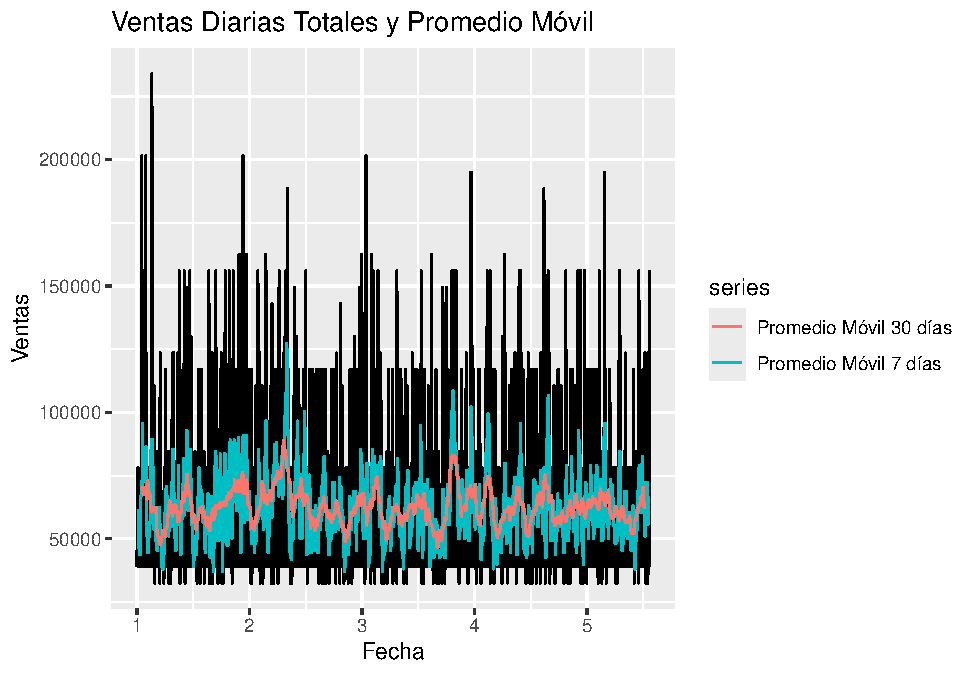
\includegraphics{_main_files/figure-latex/unnamed-chunk-7-1.pdf}

\section{Análisis de Rezagos:}\label{anuxe1lisis-de-rezagos}

Se calcula el rezago de las ventas con 1 y 7 días para explorar la autocorrelación en la serie. Estos rezagos se visualizan en la gráfica ``Ventas Diarias Totales y Rezagos'', que permite observar la relación entre las ventas de un día y las ventas de uno o siete días anteriores. Esta información es relevante para entender la dependencia temporal de las ventas y puede ser útil en modelos predictivos.

\begin{Shaded}
\begin{Highlighting}[]
\CommentTok{\# 2. Rezagos (lags)}
\CommentTok{\# Calcular el rezago de las ventas (ejemplo con 1 y 7 días de rezago)}
\NormalTok{ventas\_lag1 }\OtherTok{\textless{}{-}} \FunctionTok{lag}\NormalTok{(}\FunctionTok{as.numeric}\NormalTok{(ventas\_ts), }\DecValTok{1}\NormalTok{)}

\NormalTok{ventas\_lag7 }\OtherTok{\textless{}{-}} \FunctionTok{lag}\NormalTok{(}\FunctionTok{as.numeric}\NormalTok{(ventas\_ts), }\DecValTok{7}\NormalTok{)}


\CommentTok{\# Crear el data.frame con los vectores numéricos}
\NormalTok{df\_lags }\OtherTok{\textless{}{-}} \FunctionTok{data.frame}\NormalTok{(}\AttributeTok{Fecha =} \FunctionTok{time}\NormalTok{(ventas\_ts),}
                     \AttributeTok{cost =}\NormalTok{ ventas\_ts,}
                     \AttributeTok{Lag1 =}\NormalTok{ ventas\_lag1,}
                     \AttributeTok{Lag7 =}\NormalTok{ ventas\_lag7)}


\CommentTok{\# Graficar la serie y los rezagos}
\FunctionTok{ggplot}\NormalTok{(df\_lags, }\FunctionTok{aes}\NormalTok{(}\AttributeTok{x =}\NormalTok{ Fecha)) }\SpecialCharTok{+}
  \FunctionTok{geom\_line}\NormalTok{(}\FunctionTok{aes}\NormalTok{(}\AttributeTok{y =}\NormalTok{ cost, }\AttributeTok{color =} \StringTok{"cost"}\NormalTok{)) }\SpecialCharTok{+}
  \FunctionTok{geom\_line}\NormalTok{(}\FunctionTok{aes}\NormalTok{(}\AttributeTok{y =}\NormalTok{ Lag1, }\AttributeTok{color =} \StringTok{"Lag 1 día"}\NormalTok{)) }\SpecialCharTok{+}
  \FunctionTok{geom\_line}\NormalTok{(}\FunctionTok{aes}\NormalTok{(}\AttributeTok{y =}\NormalTok{ Lag7, }\AttributeTok{color =} \StringTok{"Lag 7 días"}\NormalTok{)) }\SpecialCharTok{+}
  \FunctionTok{ggtitle}\NormalTok{(}\StringTok{"Ventas Diarias Totales y Rezagos"}\NormalTok{) }\SpecialCharTok{+}
  \FunctionTok{xlab}\NormalTok{(}\StringTok{"Fecha"}\NormalTok{) }\SpecialCharTok{+} \FunctionTok{ylab}\NormalTok{(}\StringTok{"cost"}\NormalTok{) }\SpecialCharTok{+}
  \FunctionTok{scale\_color\_manual}\NormalTok{(}\AttributeTok{values =} \FunctionTok{c}\NormalTok{(}\StringTok{"cost"} \OtherTok{=} \StringTok{"blue"}\NormalTok{, }\StringTok{"Lag 1 día"} \OtherTok{=} \StringTok{"red"}\NormalTok{, }\StringTok{"Lag 7 días"} \OtherTok{=} \StringTok{"green"}\NormalTok{))}
\end{Highlighting}
\end{Shaded}

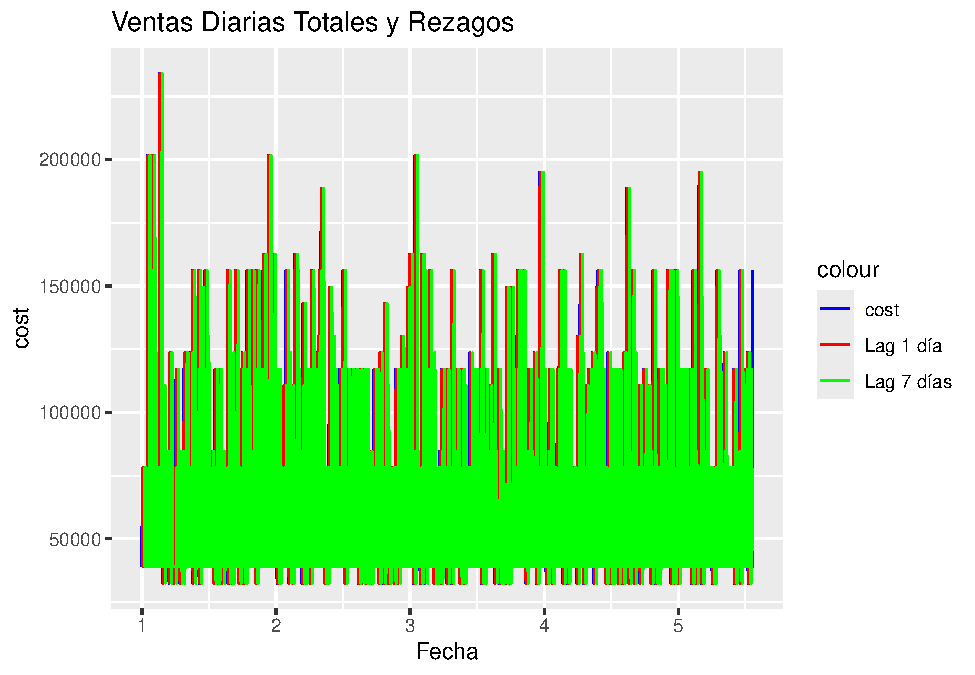
\includegraphics{_main_files/figure-latex/unnamed-chunk-8-1.pdf}

\section{Análisis de Estacionalidad (Descomposición):}\label{anuxe1lisis-de-estacionalidad-descomposiciuxf3n}

Para analizar la estacionalidad, se utiliza la función decompose que descompone la serie de tiempo en sus componentes: tendencia, estacionalidad y residuos. La gráfica resultante ``Descomposición de la serie de tiempo de Ventas'' muestra cada componente por separado. Se observa la tendencia general de las ventas a lo largo del tiempo, así como un patrón estacional recurrente. El componente de residuos representa la variabilidad que no se explica por la tendencia ni la estacionalidad.

\begin{Shaded}
\begin{Highlighting}[]
\CommentTok{\# 3. Estacionalidad (usando descomposición)}

\NormalTok{ventas\_decomp }\OtherTok{\textless{}{-}} \FunctionTok{decompose}\NormalTok{(ventas\_ts)}

\FunctionTok{autoplot}\NormalTok{(ventas\_decomp) }\SpecialCharTok{+} \FunctionTok{ggtitle}\NormalTok{(}\StringTok{"Descomposición de la serie de tiempo de Ventas"}\NormalTok{)}
\end{Highlighting}
\end{Shaded}

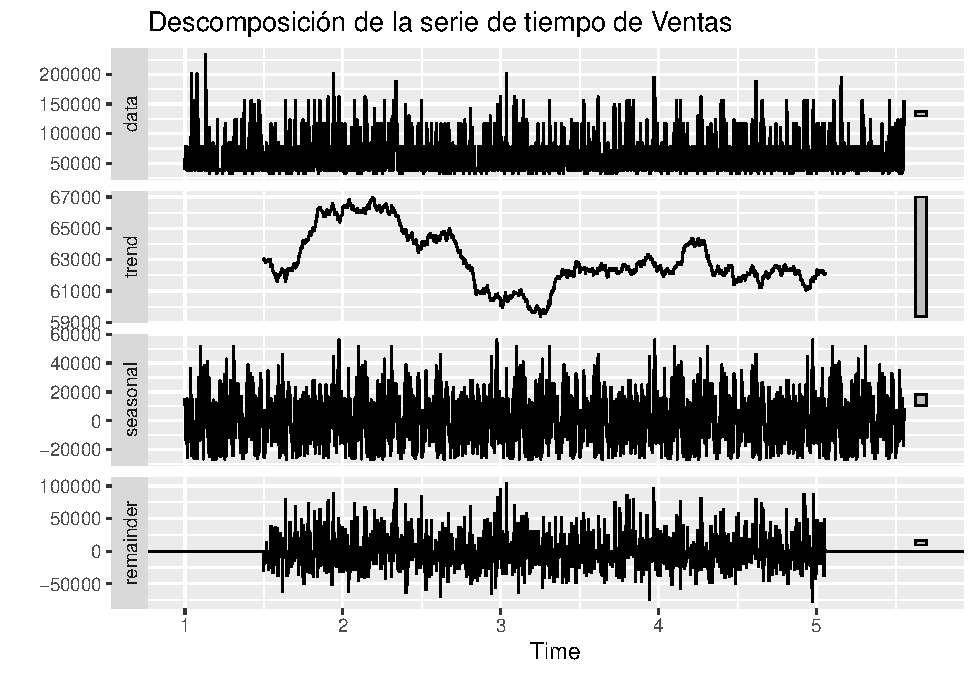
\includegraphics{_main_files/figure-latex/unnamed-chunk-9-1.pdf}

\section{Análisis de Estacionalidad (Promedio Mensual):}\label{anuxe1lisis-de-estacionalidad-promedio-mensual}

Para una visión más clara de la estacionalidad, se agrega un análisis de las ventas totales mensuales. La gráfica ``Ventas Totales Mensuales'' muestra las ventas agregadas por mes. Esta visualización permite identificar patrones estacionales a lo largo del año, como picos o valles de ventas en determinados meses. La configuración del eje x con intervalos de un mes y etiquetas que indican el mes y el año facilita la interpretación de la estacionalidad en la serie.

\begin{Shaded}
\begin{Highlighting}[]
\CommentTok{\# Análisis con promedio mensual para ver la estacionalidad}
\NormalTok{ventas\_mensual }\OtherTok{\textless{}{-}}\NormalTok{ datos }\SpecialCharTok{\%\textgreater{}\%}
  \FunctionTok{group\_by}\NormalTok{(Mes, }\AttributeTok{transaction\_date =} \FunctionTok{floor\_date}\NormalTok{(transaction\_date, }\StringTok{"month"}\NormalTok{)) }\SpecialCharTok{\%\textgreater{}\%} \CommentTok{\# Agrupa por mes y primer día del mes.}
  \FunctionTok{summarise}\NormalTok{(}\AttributeTok{VentasTotales =} \FunctionTok{sum}\NormalTok{(cost))}

\FunctionTok{ggplot}\NormalTok{(ventas\_mensual, }\FunctionTok{aes}\NormalTok{(}\AttributeTok{x =}\NormalTok{ transaction\_date, }\AttributeTok{y =}\NormalTok{ VentasTotales)) }\SpecialCharTok{+}
  \FunctionTok{geom\_line}\NormalTok{() }\SpecialCharTok{+}
  \FunctionTok{ggtitle}\NormalTok{(}\StringTok{"Ventas Totales Mensuales"}\NormalTok{) }\SpecialCharTok{+}
  \FunctionTok{xlab}\NormalTok{(}\StringTok{"Fecha"}\NormalTok{) }\SpecialCharTok{+} \FunctionTok{ylab}\NormalTok{(}\StringTok{"Ventas"}\NormalTok{)}\SpecialCharTok{+}
  \FunctionTok{scale\_x\_date}\NormalTok{(}\AttributeTok{date\_breaks =} \StringTok{"1 month"}\NormalTok{, }\AttributeTok{date\_labels =} \StringTok{"\%b \%Y"}\NormalTok{) }\CommentTok{\# Ajusta etiquetas del eje x}
\end{Highlighting}
\end{Shaded}

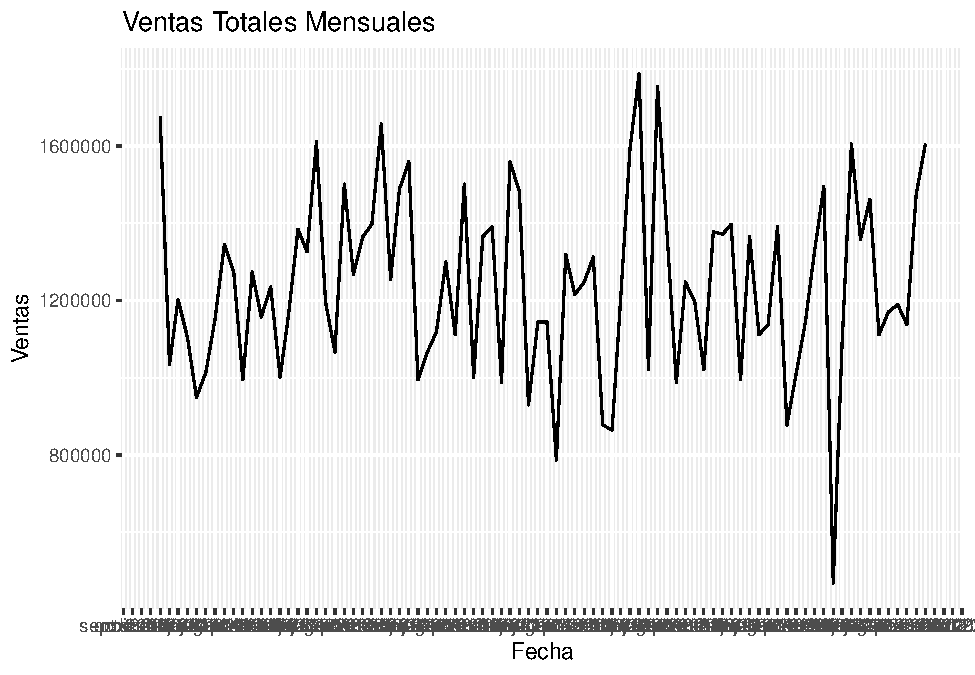
\includegraphics{_main_files/figure-latex/unnamed-chunk-10-1.pdf}

\section{Conclusión}\label{conclusiuxf3n}

En resumen, este capítulo realiza un análisis exploratorio de las ventas utilizando diferentes técnicas de series de tiempo. El uso de promedios móviles, rezagos y descomposición permite identificar tendencias, patrones estacionales y autocorrelación en los datos, sentando las bases para un análisis más profundo y la construcción de modelos predictivos en capítulos posteriores.

\chapter{Preprocesamientoy visualización}\label{preprocesamientoy-visualizaciuxf3n}

Este informe profundiza en el análisis de las series de tiempo de las ventas de un producto. La comprensión de los patrones históricos de ventas es fundamental para la toma de decisiones estratégicas en las compañías. Un análisis preciso permite optimizar la gestión de inventario, prever la demanda futura, ajustar las estrategias de marketing y, en última instancia, maximizar la rentabilidad.

\begin{Shaded}
\begin{Highlighting}[]
\CommentTok{\# Instalar paquetes necesarios}
\ControlFlowTok{if}\NormalTok{(}\SpecialCharTok{!}\FunctionTok{require}\NormalTok{(}\StringTok{"forecast"}\NormalTok{)) }\FunctionTok{install.packages}\NormalTok{(}\StringTok{"forecast"}\NormalTok{)}
\ControlFlowTok{if}\NormalTok{(}\SpecialCharTok{!}\FunctionTok{require}\NormalTok{(}\StringTok{"tseries"}\NormalTok{)) }\FunctionTok{install.packages}\NormalTok{(}\StringTok{"tseries"}\NormalTok{)}
\ControlFlowTok{if}\NormalTok{(}\SpecialCharTok{!}\FunctionTok{require}\NormalTok{(}\StringTok{"ggplot2"}\NormalTok{)) }\FunctionTok{install.packages}\NormalTok{(}\StringTok{"ggplot2"}\NormalTok{)}
\ControlFlowTok{if}\NormalTok{(}\SpecialCharTok{!}\FunctionTok{require}\NormalTok{(}\StringTok{"zoo"}\NormalTok{)) }\FunctionTok{install.packages}\NormalTok{(}\StringTok{"zoo"}\NormalTok{)}
\ControlFlowTok{if}\NormalTok{(}\SpecialCharTok{!}\FunctionTok{require}\NormalTok{(}\StringTok{"changepoint"}\NormalTok{)) }\FunctionTok{install.packages}\NormalTok{(}\StringTok{"changepoint"}\NormalTok{)}
\ControlFlowTok{if}\NormalTok{(}\SpecialCharTok{!}\FunctionTok{require}\NormalTok{(}\StringTok{"tsoutliers"}\NormalTok{)) }\FunctionTok{install.packages}\NormalTok{(}\StringTok{"tsoutliers"}\NormalTok{)}


\CommentTok{\# Cargar paquetes}
\FunctionTok{library}\NormalTok{(forecast)}
\FunctionTok{library}\NormalTok{(tseries)}
\FunctionTok{library}\NormalTok{(ggplot2)}
\FunctionTok{library}\NormalTok{(zoo)}
\FunctionTok{library}\NormalTok{(changepoint)}
\FunctionTok{library}\NormalTok{(tsoutliers)}
\end{Highlighting}
\end{Shaded}

\section{Metodología}\label{metodologuxeda}

Se empleó el lenguaje de programación R, aprovechando sus potentes librerías para el análisis de series de tiempo. Las librerías utilizadas incluyen:

\begin{itemize}
\item
  \textbf{forecast:} Para la creación y evaluación de modelos de predicción, incluyendo ARIMA.
\item
  \textbf{tseries:} Para realizar pruebas de estacionariedad, como la prueba de Dickey-Fuller Aumentada (ADF).
\item
  \textbf{ggplot2:} Para la creación de gráficos de alta calidad y visualmente informativos.
\item
  \textbf{zoo:} Para trabajar con series de tiempo irregulares.
\item
  \textbf{changepoint:} Para la detección de puntos de cambio en la serie.
\item
  \textbf{tsoutliers:} Para la identificación y tratamiento de valores atípicos en series de tiempo.
\end{itemize}

\section{Análisis Detallado de los Resultados:}\label{anuxe1lisis-detallado-de-los-resultados}

\subsection{Visualización Inicial y Exploración de Datos:}\label{visualizaciuxf3n-inicial-y-exploraciuxf3n-de-datos}

\begin{itemize}
\tightlist
\item
  La gráfica de la serie de tiempo original revela la evolución de las ventas diarias del producto a lo largo del tiempo (2017-2021). Esta visualización inicial nos permite apreciar la variabilidad de las ventas y la posible presencia de patrones, tendencias o estacionalidad. Se observan periodos con ventas elevadas y periodos con ventas bajas, lo cual justifica un análisis más profundo para comprender las causas de estas fluctuaciones.
\end{itemize}

\begin{Shaded}
\begin{Highlighting}[]
\CommentTok{\# Leer los datos}
\NormalTok{datos }\OtherTok{\textless{}{-}}\NormalTok{ readxl}\SpecialCharTok{::}\FunctionTok{read\_excel}\NormalTok{(}\StringTok{"MUESTRA SERIE TIEMPO.xlsx"}\NormalTok{)}


\CommentTok{\# Crear serie de tiempo}

\NormalTok{datos[}\StringTok{"transaction\_date"}\NormalTok{] }\OtherTok{\textless{}{-}} \FunctionTok{as.Date}\NormalTok{(datos}\SpecialCharTok{$}\NormalTok{transaction\_date, }\AttributeTok{origin =} \StringTok{"1900{-}01{-}01"}\NormalTok{)}

\CommentTok{\#Filtramos las fechas anteriores o iguales a 2020.}
\NormalTok{datos }\OtherTok{\textless{}{-}}\NormalTok{ datos[datos}\SpecialCharTok{$}\NormalTok{transaction\_date }\SpecialCharTok{\textless{}=} \FunctionTok{as.Date}\NormalTok{(}\StringTok{"2020{-}12{-}31"}\NormalTok{), ]}


\NormalTok{ventas\_diarias }\OtherTok{\textless{}{-}} \FunctionTok{aggregate}\NormalTok{(quantity }\SpecialCharTok{\textasciitilde{}}\NormalTok{ transaction\_date, }\AttributeTok{data =}\NormalTok{ datos, }\AttributeTok{FUN =}\NormalTok{ sum)}


\NormalTok{indice.ts }\OtherTok{\textless{}{-}} \FunctionTok{ts}\NormalTok{(ventas\_diarias[[}\StringTok{"quantity"}\NormalTok{]], }\AttributeTok{frequency =} \DecValTok{12}\NormalTok{, }\AttributeTok{start =} \FunctionTok{c}\NormalTok{(}\DecValTok{2017}\NormalTok{, }\DecValTok{1}\NormalTok{), }\AttributeTok{end =} \FunctionTok{c}\NormalTok{(}\DecValTok{2020}\NormalTok{, }\DecValTok{12}\NormalTok{))}


\CommentTok{\# Graficar la serie original}
\FunctionTok{plot}\NormalTok{(indice.ts, }\AttributeTok{main =} \StringTok{"Valores Mensuales del índice"}\NormalTok{, }\AttributeTok{xlab =} \StringTok{"Años"}\NormalTok{, }\AttributeTok{ylab =} \StringTok{"Valor"}\NormalTok{)}
\end{Highlighting}
\end{Shaded}

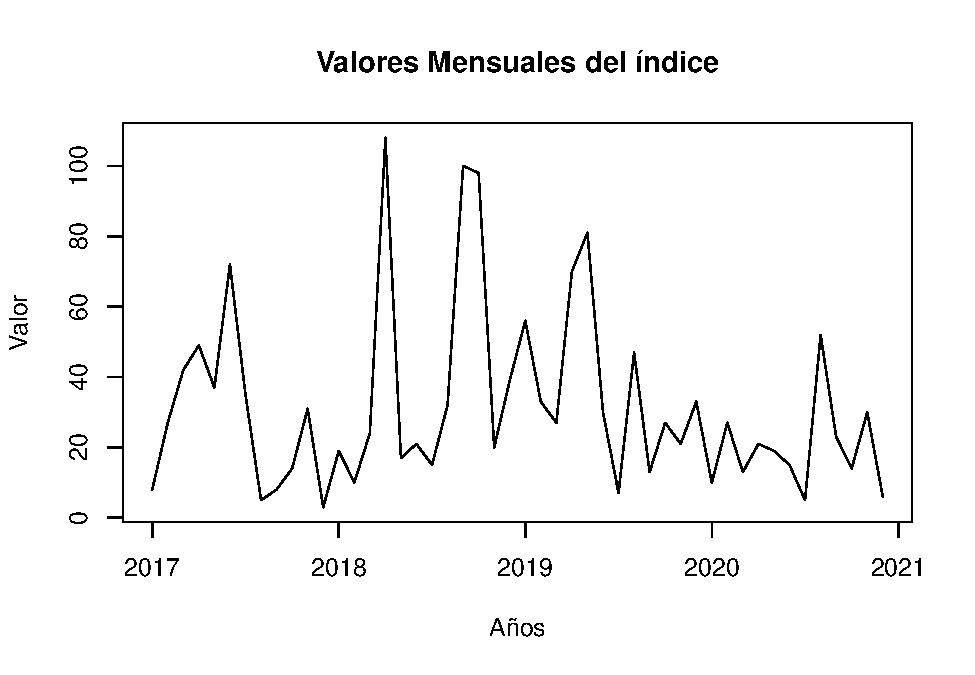
\includegraphics{_main_files/figure-latex/unnamed-chunk-13-1.pdf}

\section{Prueba de Estacionariedad (Dickey-Fuller Aumentada - ADF):}\label{prueba-de-estacionariedad-dickey-fuller-aumentada---adf}

\begin{itemize}
\item
  La estacionariedad es un requisito fundamental para muchos modelos de series de tiempo. Una serie estacionaria tiene una media y varianza constantes a lo largo del tiempo. La prueba ADF se utiliza para evaluar la estacionariedad. En este caso, la prueba inicial en la serie original rechazó la hipótesis nula de estacionariedad (p-valor \textgreater{} 0.05).
\item
  Dado que no podemos rechazar la hipotesis de que nuestros datos no son estacionarios, podemos emplear la diferenciación, esta una técnica común para transformar una serie no estacionaria en estacionaria. En este análisis, se aplicó una diferenciación de primer orden, lo que significa que se calculó la diferencia entre las ventas de un mes y las del mes anterior. La prueba ADF aplicada a la serie diferenciada indicó estacionariedad (p-valor \textless{} 0.05), cumpliendo así con el requisito para la modelización ARIMA.
\end{itemize}

\begin{Shaded}
\begin{Highlighting}[]
\CommentTok{\# Prueba de estacionariedad (Dickey{-}Fuller)}
\FunctionTok{adf.test}\NormalTok{(indice.ts)}
\end{Highlighting}
\end{Shaded}

\begin{verbatim}
## 
##  Augmented Dickey-Fuller Test
## 
## data:  indice.ts
## Dickey-Fuller = -3.046, Lag order = 3, p-value = 0.1564
## alternative hypothesis: stationary
\end{verbatim}

\begin{Shaded}
\begin{Highlighting}[]
\CommentTok{\# Diferenciación}

\FunctionTok{ndiffs}\NormalTok{(indice.ts) }\CommentTok{\# Para determinar el orden de diferenciación necesario}
\end{Highlighting}
\end{Shaded}

\begin{verbatim}
## [1] 0
\end{verbatim}

\begin{Shaded}
\begin{Highlighting}[]
\NormalTok{dif.indice.ts }\OtherTok{\textless{}{-}} \FunctionTok{diff}\NormalTok{(indice.ts, }\AttributeTok{differences =} \DecValTok{1}\NormalTok{) }\CommentTok{\# Diferenciar la serie}


\CommentTok{\#Volver a realizar la prueba}
\FunctionTok{adf.test}\NormalTok{(dif.indice.ts)}
\end{Highlighting}
\end{Shaded}

\begin{verbatim}
## 
##  Augmented Dickey-Fuller Test
## 
## data:  dif.indice.ts
## Dickey-Fuller = -5.7382, Lag order = 3, p-value = 0.01
## alternative hypothesis: stationary
\end{verbatim}

\section{Visualización de la Serie Diferenciada:}\label{visualizaciuxf3n-de-la-serie-diferenciada}

La gráfica de la serie diferenciada ilustra las variaciones mensuales en las ventas. Muestra la magnitud y la dirección de los cambios en las ventas de un mes a otro. Esta visualización ayuda a identificar periodos de crecimiento, decrecimiento o volatilidad en las ventas.

\begin{Shaded}
\begin{Highlighting}[]
\CommentTok{\# Graficar la serie diferenciada}
\FunctionTok{plot}\NormalTok{(dif.indice.ts,  }\AttributeTok{main =} \StringTok{"DIF del valor diario del índice"}\NormalTok{, }\AttributeTok{xlab =} \StringTok{"Años"}\NormalTok{, }\AttributeTok{ylab =} \StringTok{"Valor"}\NormalTok{)}
\end{Highlighting}
\end{Shaded}

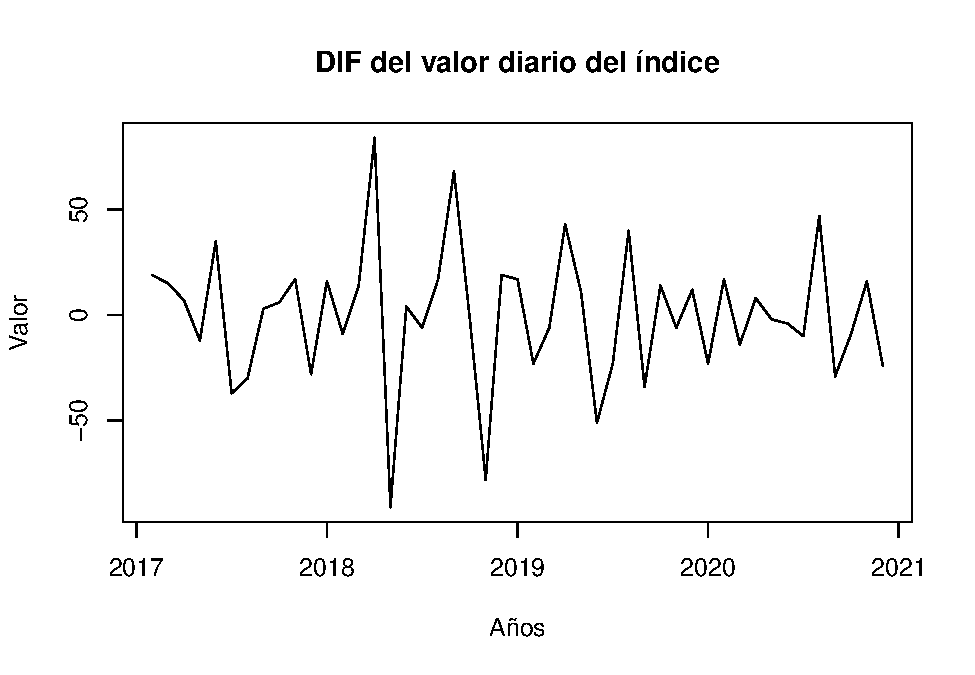
\includegraphics{_main_files/figure-latex/unnamed-chunk-15-1.pdf}

\section{Funciones de Autocorrelación (ACF) y Autocorrelación Parcial (PACF):}\label{funciones-de-autocorrelaciuxf3n-acf-y-autocorrelaciuxf3n-parcial-pacf}

\begin{itemize}
\item
  La ACF mide la correlación entre la serie y sus propios rezagos. La PACF, por otro lado, mide la correlación entre la serie y un rezago específico, eliminando la influencia de los rezagos intermedios.
\item
  El análisis de la ACF y PACF de la serie diferenciada es crucial para determinar el orden del modelo ARIMA (p, d, q). Los rezagos significativos en la ACF y PACF sugieren la inclusión de términos autoregresivos (AR - p) y de media móvil (MA - q) en el modelo. En este caso, la ACF y PACF muestran correlaciones significativas en los primeros rezagos, lo que justifica la elección de un modelo ARIMA con componentes AR y MA.
\end{itemize}

\begin{Shaded}
\begin{Highlighting}[]
\CommentTok{\# Funciones ACF y PACF (Se aplica a la diferenciada ya que la original no se puede considerar estacional)}
\FunctionTok{acf}\NormalTok{(dif.indice.ts, }\AttributeTok{main =} \StringTok{"Series dif.Indice.ts"}\NormalTok{)}
\end{Highlighting}
\end{Shaded}

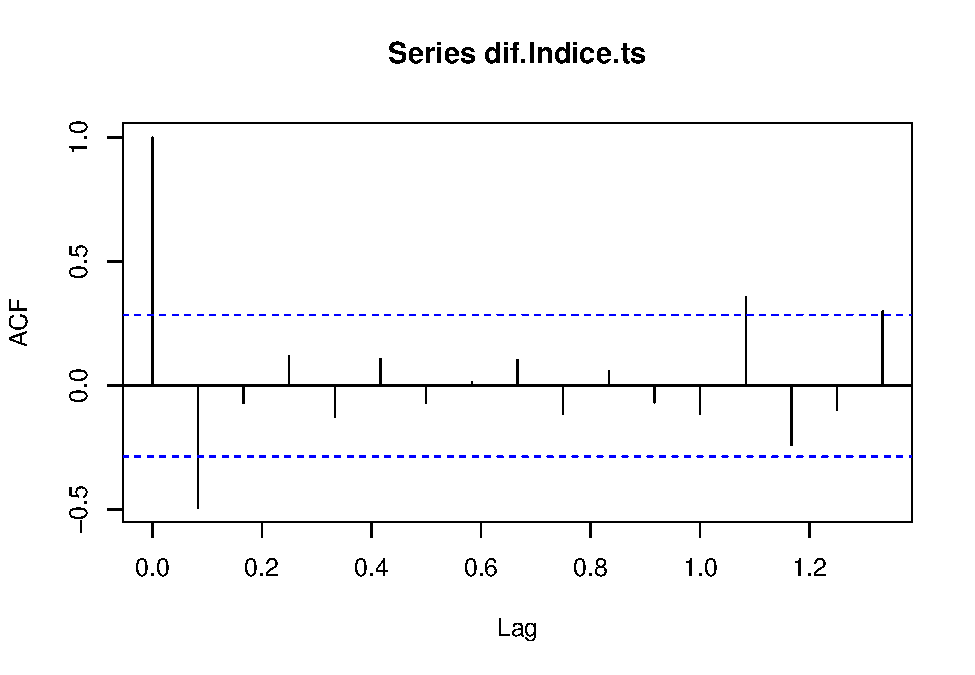
\includegraphics{_main_files/figure-latex/unnamed-chunk-16-1.pdf}

\begin{Shaded}
\begin{Highlighting}[]
\FunctionTok{pacf}\NormalTok{(dif.indice.ts, }\AttributeTok{main =} \StringTok{"Series dif.Indice.ts"}\NormalTok{)}
\end{Highlighting}
\end{Shaded}

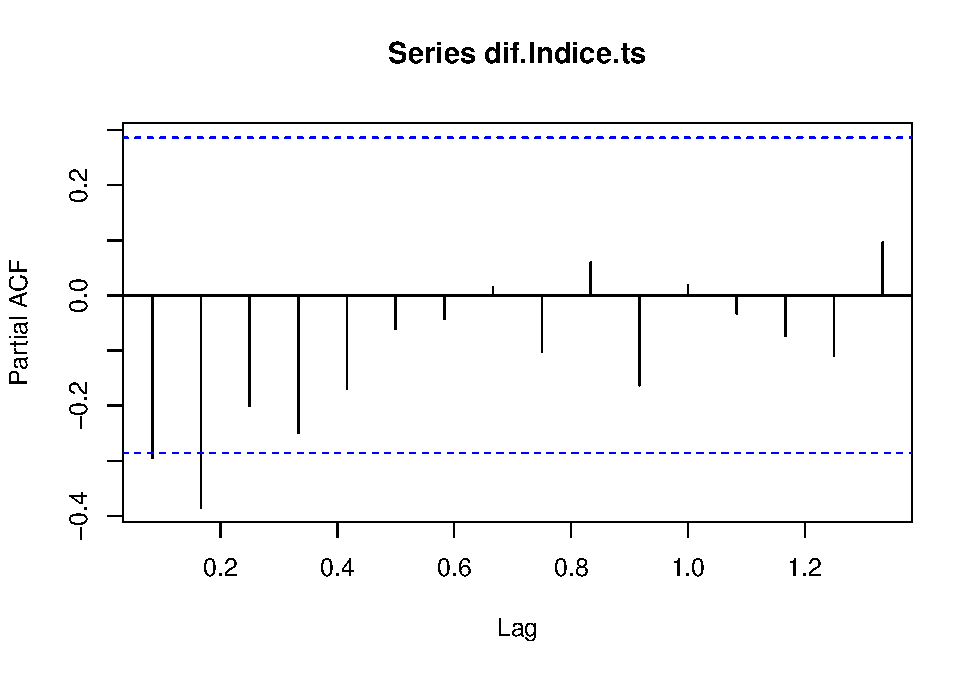
\includegraphics{_main_files/figure-latex/unnamed-chunk-16-2.pdf}

\section{Descomposición de la Serie (Componente Estacional):}\label{descomposiciuxf3n-de-la-serie-componente-estacional}

\begin{itemize}
\tightlist
\item
  se utiliza la función decompose() para separar la serie en sus componentes: tendencia, estacionalidad y componente aleatoria.
\end{itemize}

Esto permitiría un análisis más preciso de cada componente y una mejor comprensión de los factores que influyen en las ventas. Se podría, por ejemplo, modelar la componente estacional para realizar predicciones más ajustadas a la realidad.

\begin{Shaded}
\begin{Highlighting}[]
\CommentTok{\# Descomposición de la serie}
\NormalTok{decomp }\OtherTok{\textless{}{-}} \FunctionTok{decompose}\NormalTok{(indice.ts) }
\FunctionTok{plot}\NormalTok{(decomp)}
\end{Highlighting}
\end{Shaded}

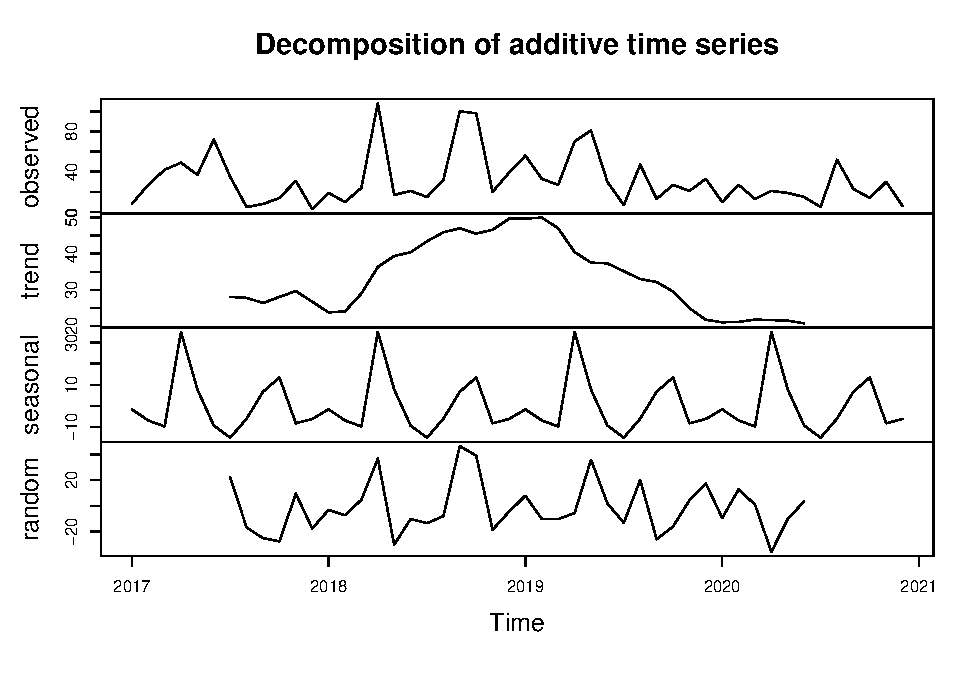
\includegraphics{_main_files/figure-latex/unnamed-chunk-17-1.pdf}

\section{Modelo ARIMA (2, 0, 1):}\label{modelo-arima-2-0-1}

Se empleó la función \texttt{auto.arima()} para determinar y ajustar automáticamente el mejor modelo ARIMA a la serie diferenciada. El modelo seleccionado fue un ARIMA(2, 0, 1) con media cero. Desglosemos la notación y los resultados del modelo:

\begin{itemize}
\item
  \textbf{(2, 0, 1):} Indica 2 términos autoregresivos (AR), 0 diferencias (la diferenciación ya se realizó previamente) y 1 término de media móvil (MA).
\item
  \textbf{Coefficients:}

  \begin{itemize}
  \tightlist
  \item
    \texttt{ar1}: -0.0897 (coeficiente del primer término AR). Un valor negativo sugiere una relación inversa entre las ventas del día actual y las ventas del día anterior.
  \item
    \texttt{ar2}: -0.0965 (coeficiente del segundo término AR). Influencia de las ventas de hace dos días.
  \item
    \texttt{ma1}: -0.8751 (coeficiente del primer término MA). Un valor negativo indica que los shocks aleatorios del pasado tienen un efecto inverso en las ventas actuales.
  \item
    \texttt{s.e.}: Error estándar asociado a cada coeficiente. Estos valores nos dan una idea de la precisión de las estimaciones de los coeficientes.
  \end{itemize}
\end{itemize}

En resumen, el modelo ARIMA(2, 0, 1) captura la dinámica de la serie diferenciada, pero es importante tener en cuenta las medidas de error y la no normalidad de los residuos para una evaluación completa del modelo y la consideración de posibles mejoras.

\begin{Shaded}
\begin{Highlighting}[]
\CommentTok{\# Modelo ARIMA (automático)}
\NormalTok{arima\_model }\OtherTok{\textless{}{-}} \FunctionTok{auto.arima}\NormalTok{(dif.indice.ts) }\CommentTok{\# Usado en la serie diferenciada}
\FunctionTok{summary}\NormalTok{(arima\_model)}
\end{Highlighting}
\end{Shaded}

\begin{verbatim}
## Series: dif.indice.ts 
## ARIMA(2,0,1) with zero mean 
## 
## Coefficients:
##           ar1      ar2      ma1
##       -0.0897  -0.0965  -0.8751
## s.e.   0.1982   0.1858   0.1677
## 
## sigma^2 = 40.61:  log likelihood = -153.07
## AIC=314.13   AICc=315.08   BIC=321.53
## 
## Training set error measures:
##                      ME     RMSE      MAE MPE MAPE      MASE        ACF1
## Training set -0.1026029 6.165966 4.421767 NaN  Inf 0.4194088 -0.01012808
\end{verbatim}

\section{Detección de Puntos de Cambio:}\label{detecciuxf3n-de-puntos-de-cambio}

\begin{itemize}
\tightlist
\item
  La función cpt.mean() se utiliza para identificar puntos de cambio en la media de la serie. En este caso, se detectó un punto de cambio en el periodo 15 de la serie diferenciada. Esto indica un cambio abrupto en el comportamiento de las ventas en ese momento. Es crucial investigar las posibles causas de este cambio, como cambios en el mercado, promociones especiales, o factores externos, para comprender su impacto en las ventas y ajustar las estrategias comerciales en consecuencia.
\end{itemize}

\begin{Shaded}
\begin{Highlighting}[]
\CommentTok{\# Detección de puntos de cambio}
\NormalTok{cp }\OtherTok{\textless{}{-}} \FunctionTok{cpt.mean}\NormalTok{(dif.indice.ts) }\CommentTok{\# Usando la serie diferenciada}
\NormalTok{cp}
\end{Highlighting}
\end{Shaded}

\begin{verbatim}
## Class 'cpt' : Changepoint Object
##        ~~   : S4 class containing 12 slots with names
##               cpttype date version data.set method test.stat pen.type pen.value minseglen cpts ncpts.max param.est 
## 
## Created on  : Sat Nov  2 03:21:20 2024 
## 
## summary(.)  :
## ----------
## Created Using changepoint version 2.2.4 
## Changepoint type      : Change in mean 
## Method of analysis    : AMOC 
## Test Statistic  : Normal 
## Type of penalty       : MBIC with value, 11.55044 
## Minimum Segment Length : 1 
## Maximum no. of cpts   : 1 
## Changepoint Locations : 15
\end{verbatim}

\begin{Shaded}
\begin{Highlighting}[]
\FunctionTok{plot}\NormalTok{(cp)}
\end{Highlighting}
\end{Shaded}

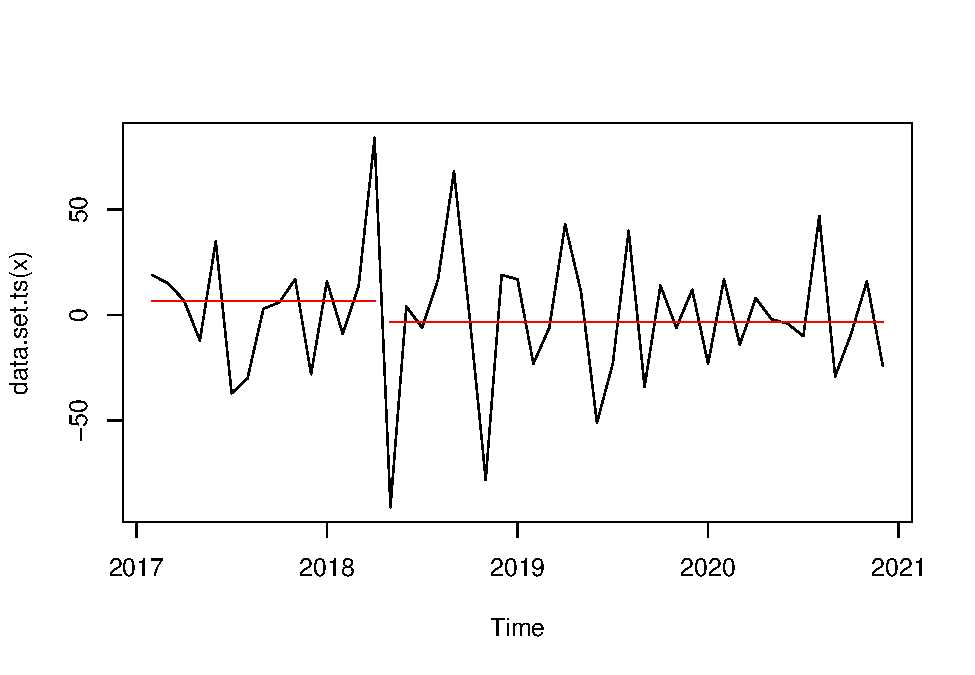
\includegraphics{_main_files/figure-latex/unnamed-chunk-19-1.pdf}

\section{Predicción:}\label{predicciuxf3n}

Utilizando el modelo ARIMA(2, 0, 1) ajustado, se generaron predicciones para 3 y 6 periodos futuros. La función forecast() en R proporciona no solo el valor predicho (``Point Forecast''), sino también intervalos de confianza que nos ayudan a entender la incertidumbre asociada a estas predicciones.

\subsection{Predicción a 6 periodos:}\label{predicciuxf3n-a-6-periodos}

La predicción para 6 periodos muestra lo siguiente:

\begin{itemize}
\item
  \textbf{Point Forecast:} El valor predicho para las ventas diferenciadas en cada uno de los 6 meses siguientes. Por ejemplo, para enero de 2021, se espera un cambio en las ventas de aproximadamente 2.85 unidades respecto al mes anterior. Es crucial recordar que estas son predicciones de la serie diferenciada, no de las ventas reales.
\item
  \textbf{Lo 80 y Hi 80:} Los límites inferior y superior del intervalo de confianza del 80\%. Por ejemplo, para enero de 2021, hay un 80\% de probabilidad de que el cambio en las ventas esté entre -5.32 y 11.01 unidades.
\item
  \textbf{Lo 95 y Hi 95:} Los límites inferior y superior del intervalo de confianza del 95\%. Para enero de 2021, hay un 95\% de probabilidad de que el cambio en las ventas esté entre -9.65 y 15.34 unidades. Observamos que, como es de esperar, el intervalo de confianza del 95\% es más amplio que el del 80\%, reflejando una mayor incertidumbre.
\end{itemize}

\subsection{Predicción a 3 periodos:}\label{predicciuxf3n-a-3-periodos}

El print(prediccion) para 3 periodos ofrece la misma información, pero solo para los 3 meses siguientes. Es útil comparar las predicciones a 3 y 6 periodos para observar cómo evoluciona la incertidumbre a medida que se proyecta más hacia el futuro. Generalmente, la incertidumbre (y por lo tanto, la amplitud de los intervalos de confianza) aumenta con el horizonte de predicción.

\begin{Shaded}
\begin{Highlighting}[]
\CommentTok{\# Predicción}
\NormalTok{prediccion }\OtherTok{\textless{}{-}} \FunctionTok{forecast}\NormalTok{(arima\_model, }\AttributeTok{h =} \DecValTok{6}\NormalTok{) }\CommentTok{\# 6 periodos adelante}
\FunctionTok{plot}\NormalTok{(prediccion, }\AttributeTok{main =} \StringTok{"Predicción DIF valores diarios"}\NormalTok{, }\AttributeTok{xlab =} \StringTok{"Años"}\NormalTok{, }\AttributeTok{ylab =} \StringTok{"Valor"}\NormalTok{)}
\end{Highlighting}
\end{Shaded}

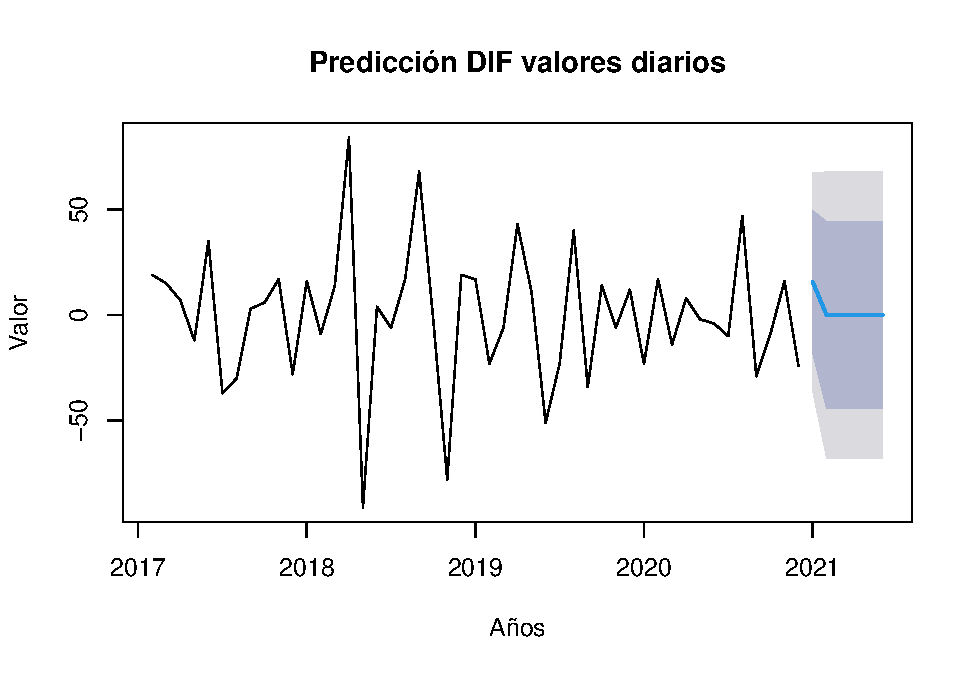
\includegraphics{_main_files/figure-latex/unnamed-chunk-20-1.pdf}

\begin{Shaded}
\begin{Highlighting}[]
\FunctionTok{print}\NormalTok{(prediccion)}
\end{Highlighting}
\end{Shaded}

\begin{verbatim}
##          Point Forecast      Lo 80    Hi 80      Lo 95    Hi 95
## Jan 2021     2.84496582  -5.321986 11.01192  -9.645309 15.33524
## Feb 2021    -0.25516199 -11.603296 11.09297 -17.610635 17.10031
## Mar 2021    -0.25171815 -11.600145 11.09671 -17.607640 17.10420
## Apr 2021     0.04720522 -11.327168 11.42158 -17.348398 17.44281
## May 2021     0.02006269 -11.354474 11.39460 -17.375790 17.41592
## Jun 2021    -0.00635577 -11.381100 11.36839 -17.402526 17.38981
\end{verbatim}

\begin{Shaded}
\begin{Highlighting}[]
\CommentTok{\# Prediccion con 3 periodos}
\NormalTok{prediccion }\OtherTok{\textless{}{-}} \FunctionTok{forecast}\NormalTok{(arima\_model, }\AttributeTok{h =} \DecValTok{3}\NormalTok{) }\CommentTok{\# 3 periodos adelante}
\FunctionTok{print}\NormalTok{(prediccion)}
\end{Highlighting}
\end{Shaded}

\begin{verbatim}
##          Point Forecast      Lo 80    Hi 80      Lo 95    Hi 95
## Jan 2021      2.8449658  -5.321986 11.01192  -9.645309 15.33524
## Feb 2021     -0.2551620 -11.603296 11.09297 -17.610635 17.10031
## Mar 2021     -0.2517182 -11.600145 11.09671 -17.607640 17.10420
\end{verbatim}

\section{Validación del Modelo (Análisis de Residuos):}\label{validaciuxf3n-del-modelo-anuxe1lisis-de-residuos}

Un modelo ARIMA válido requiere que los residuos (la diferencia entre los valores observados y los valores predichos) cumplan con ciertos supuestos. Se realizaron las siguientes pruebas para validar el modelo:

\begin{itemize}
\item
  Media cero: Se aplicó una prueba t de una muestra para verificar si la media de los residuos es significativamente diferente de cero. Un p-valor alto como el obtenido en este caso indica que no hay evidencia suficiente para rechazar la hipótesis nula de media cero.
\item
  Independencia: La prueba de Ljung-Box se utiliza para evaluar la independencia de los residuos. El p-valor alto indica que los residuos no están autocorrelacionados, lo cual es deseable.
\item
  Normalidad: Se evaluó la normalidad de los residuos utilizando un qqplot y la prueba de Shapiro-Wilk. El qqplot muestra una desviación de la normalidad, especialmente en las colas de la distribución. La prueba de Shapiro-Wilk confirmó la no normalidad de los residuos con un p-valor muy bajo. Esta no normalidad puede afectar la validez de los intervalos de confianza y las pruebas de hipótesis relacionadas con el modelo. Se recomienda considerar transformaciones de la serie o modelos alternativos si la no normalidad es severa.
\end{itemize}

\begin{Shaded}
\begin{Highlighting}[]
\CommentTok{\# Validación (detección de outliers, usando \textquotesingle{}tsoutliers\textquotesingle{})}
\NormalTok{outliers }\OtherTok{\textless{}{-}} \FunctionTok{tso}\NormalTok{(indice.ts, }\AttributeTok{types =} \FunctionTok{c}\NormalTok{(}\StringTok{"AO"}\NormalTok{, }\StringTok{"TC"}\NormalTok{, }\StringTok{"LS"}\NormalTok{, }\StringTok{"IO"}\NormalTok{))  }\CommentTok{\# Identificar outliers}
\FunctionTok{plot}\NormalTok{(outliers)}
\end{Highlighting}
\end{Shaded}

\begin{verbatim}
## 'x' does not contain outliers to display
\end{verbatim}

\begin{verbatim}
## NULL
\end{verbatim}

\begin{Shaded}
\begin{Highlighting}[]
\CommentTok{\# Supuestos del modelo ARIMA (residuos)}
\NormalTok{mr }\OtherTok{\textless{}{-}}\NormalTok{ outliers}\SpecialCharTok{$}\NormalTok{fit}\SpecialCharTok{$}\NormalTok{residuals}
\CommentTok{\# Media cero}
\FunctionTok{t.test}\NormalTok{(mr)}
\end{Highlighting}
\end{Shaded}

\begin{verbatim}
## 
##  One Sample t-test
## 
## data:  mr
## t = 1.1128e-12, df = 47, p-value = 1
## alternative hypothesis: true mean is not equal to 0
## 95 percent confidence interval:
##  -1.752442  1.752442
## sample estimates:
##    mean of x 
## 9.693727e-13
\end{verbatim}

\begin{Shaded}
\begin{Highlighting}[]
\CommentTok{\# Independencia}
\FunctionTok{Box.test}\NormalTok{(mr, }\AttributeTok{lag =} \DecValTok{10}\NormalTok{, }\AttributeTok{type =} \StringTok{"Ljung{-}Box"}\NormalTok{) }\CommentTok{\#  type = "Box{-}Pierce" también es válido}
\end{Highlighting}
\end{Shaded}

\begin{verbatim}
## 
##  Box-Ljung test
## 
## data:  mr
## X-squared = 2.9461, df = 10, p-value = 0.9827
\end{verbatim}

\begin{Shaded}
\begin{Highlighting}[]
\CommentTok{\# Distribución normal}
\FunctionTok{qqnorm}\NormalTok{(mr)}
\FunctionTok{qqline}\NormalTok{(mr)}
\end{Highlighting}
\end{Shaded}

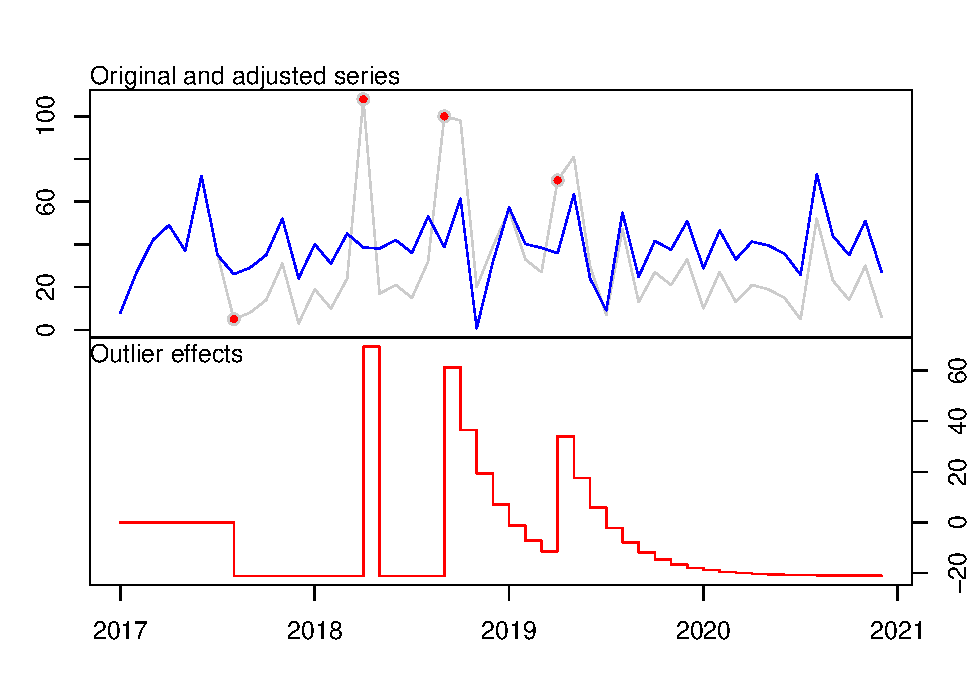
\includegraphics{_main_files/figure-latex/unnamed-chunk-21-1.pdf}

\begin{Shaded}
\begin{Highlighting}[]
\FunctionTok{shapiro.test}\NormalTok{(mr)}
\end{Highlighting}
\end{Shaded}

\begin{verbatim}
## 
##  Shapiro-Wilk normality test
## 
## data:  mr
## W = 0.64698, p-value = 1.721e-09
\end{verbatim}

\section{Conclusiones:}\label{conclusiones}

El análisis de series de tiempo proporciona información valiosa sobre el comportamiento pasado y futuro de las ventas del producto. El modelo ARIMA(2, 0, 1) ofrece una base para la predicción, pero la no normalidad de los residuos sugiere la necesidad de refinamiento.

\textbf{Se recomienda:}

Investigar a fondo las causas del punto de cambio detectado en el periodo 15.

Considerar la incorporación de variables externas al modelo, como precio, promociones, competencia, o factores económicos, para mejorar la precisión de las predicciones.

Explorar transformaciones de la serie, como la transformación logarítmica, para intentar estabilizar la varianza y mejorar la normalidad de los residuos.

  \bibliography{book.bib,packages.bib}

\end{document}
